\documentclass{article}
\usepackage{amsmath}
\usepackage{graphicx}
\usepackage{float}
\usepackage{fancyhdr}
\usepackage[spanish]{babel}
\usepackage[utf8]{inputenc}
\usepackage[justification=centering]{caption}
\usepackage[font={small}]{caption}

\setlength{\headheight}{15pt}
\parindent 0em
\parskip 2ex
\pagestyle{fancy}
\setlength{\textfloatsep}{5pt}

\newcommand{\forceindent}{\leavevmode{\parindent=1em\indent}}


\begin{document}

\begin{titlepage}
\newcommand{\HRule}{\rule{\linewidth}{0.5mm}}

\center
\textsc{\LARGE ITESO, Universidad Jesuita De Guadalajara}\\[2cm]
\textsc{\Large INGENIERÍA FINANCIERA}\\[1cm]
\textsc{\large Innovación y Gestión De Proyectos}\\[1cm]
\HRule \\[2cm]
{ \huge \bfseries Accidentes viales en la Zona Metropolitana de Guadalajara}\\[2cm]
\HRule \\[2cm]
\begin{minipage}{0.4\textwidth}
\begin{flushleft} \large


\emph{Autores:}\\
\small Alicia Karime González Beltrán\\
\small Ana Goretti Chávez Flores\\
\small Rodrigo Hernández Mota\\
\small José Felipe Sánchez Andaluz
\end{flushleft}
\end{minipage}
~
\begin{minipage}{0.4\textwidth}
\begin{flushright} \large
\emph{Supervisor:} \\
\small Mtra. Mireya \textsc{Pasillas Torres}
\end{flushright}
\end{minipage}\\[2cm]

{\large \today}\\[1cm]

\vfill
 
\end{titlepage}
\tableofcontents
\newpage

\section{Introducción}\label{sec:into}
[agregar contenido]

\newpage
\section{Diagnóstico}\label{sec:diagnostic}

Datos provenientes de la Secretaría de Movilidad de Jalisco (SEMOV) señalan que en 2016 se generaron
más de \textbf{23,753 accidentes viales} dentro de la Zona Metropolitana de
Guadalajara (ZMG). Esta cifra corresponde al 93\% de todos los accidentes
viales de todo el estado. Aunado a esto, el INEGI reporta 3,429,847
vehículos en circulación en el estado durante este mismo año. Esto significa que de cada 1000 vehículos
se generaron 7 accidentes viales en promedio.


Es imperativo señalar que los accidentes automovilísticos se caracterizan por provocar fuertes
repercusiones económicas para los involucrados. Adicionalmente, cifras publicadas por la
Asociación Mexicana de Instituciones de Seguros (AMIS) indican que solo el 27\% del parque vehicular en
México está asegurado. Esto representa un fuerte riesgo financiero potencial para la población con
vehículo en circulación.

El Estado de Jalisco, reconociendo la importancia de atender este problema,
ha realizado acciones para disminuir el número de accidentes viales.
Las políticas y soluciones que se han implementado muestran un efecto deseable en el cual
se percibe un decrecimiento real en el número de accidentes (dado que el parque vehicular ha aumentado
durante el mismo periodo de tiempo). A continuación se muestra una gráfica con el número
de accidentes viales total por año dentro de la ZMG.

	\begin{figure}[H]\centering
	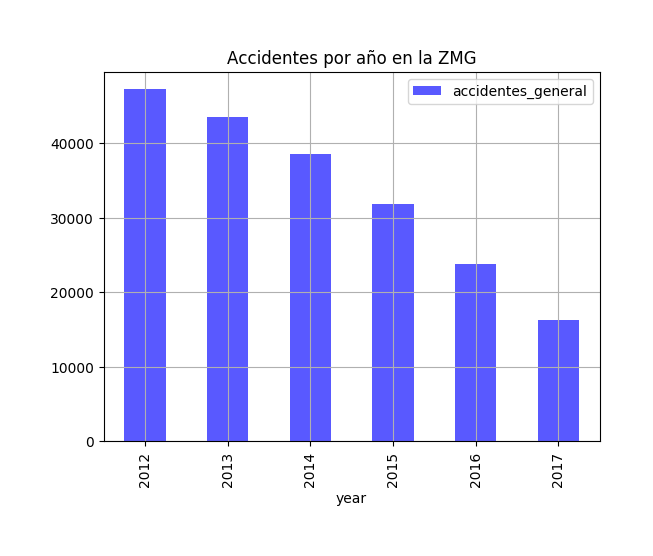
\includegraphics[width=0.60\textwidth]{resources/img/accidentes_general_img.png}
	\caption{\label{fig:accidentes_general_img} Número de accidentes viales por año dentro de la zona metropolitana de Guadalajara. Fuente: adaptación de datos de SEMOV.}
    \end{figure}

Estas políticas muestran un rendimiento excepcional en la reducción de muertes ocasionados por consumo de bebidas alcoholicas,
en donde el efecto más significativo se puede apreciar en el último año de la serie de tiempo.


	\begin{figure}[H]\centering
	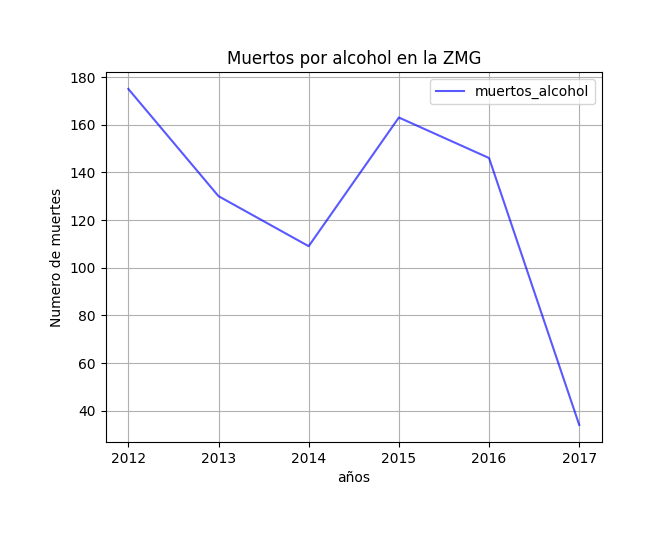
\includegraphics[width=0.60\textwidth]{resources/img/muertos_alcohol_img.png}
	\caption{\label{fig:muertes_img} Número de muertes por consumo de bebidas alcohólicas dentro de la zona metropolitana de Guadalajara. Fuente: adaptación de datos de SEMOV.}
    \end{figure}


Al analizar otras variables, es posible detectar que en general la tendencia ha sido negativa.
En particular, es de especial interés mostrar la evolución del numero de accidentes por las
categorías de lesionados involucrados, muertes total, y muertes en lugar de accidente.

	\begin{figure}[H]\centering
	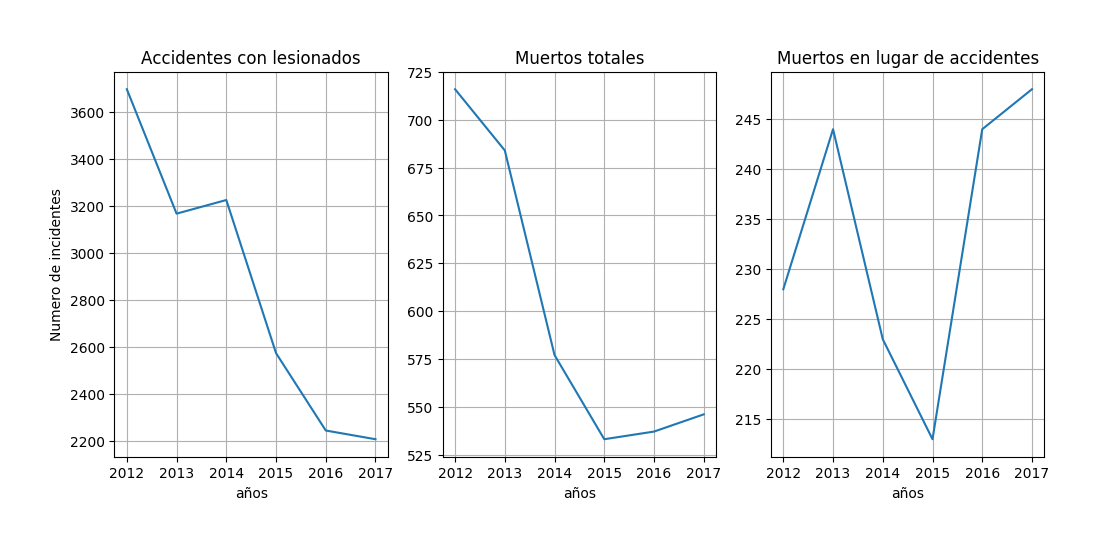
\includegraphics[width=1\textwidth]{resources/img/accidentes_general_segregacion_img.png}
	\caption{\label{fig:accidentes_general_segregacion_img} Segregación de accidentes viales dentro de la ZMG por lesionados, muertos y muertos en el lugar de accidente. Fuente: adaptación de datos de SEMOV.}
    \end{figure}

Aunque el número total de accidentes ha disminuido en forma significativa,
no todos los niveles de segregación que lo conforman presentan una disminución.
Adquiere relevancia identificar en qué segmentos la actual política de SEMOV presenta
resultados deseables y aquellos cuya situación es inmune a estas.
En este caso, se puede observar que el número de muertes en el lugar del accidente
vial ha incrementado de forma alarmante. Las causas de esto pueden variar desde
velocidad de reacción de servicios médicos, condiciones del impacto, muerte instantánea,
etc.

Una auditoría sobre la seguridad vial en la ZMG realizada por la SEMOV en colaboración con la Universidad de Guadalajara
identifica que entre los problemas de seguridad relevantes se encuentran:

	\begin{itemize}
		\item Desgaste natural del balizamiento.
		\item Falta de señales viales o en mal estado.
		\item Insuficientes espacios destinados a la circulación peatonal.
	\end{itemize}

Por otra parte, la SEMOV en su reporte ``Zonas de Riesgo'' clasifica a las causas de accidente viales en:

	\begin{itemize}
		\item Falta de distancia de seguridad.
		\item Invadir carril contrario.
		\item Virar indebidamente.
		\item No respetar señalamiento.
		\item No respetar semáforos.
		\item Exceder límites de velocidad.
		\item Rebaso indebido.
		\item Falla mecánica del vehículo.
		\item Exceso de carga o dimensiones.
		\item Circular en sentido contrario.
		\item Falta de señalamiento.
		\item Dormitar.
	\end{itemize}


Este estudio propone el siguiente árbol de problemas (véase Figura \ref{fig:arbol}) con el fin de identificar las causas y consecuencias que desencadena el tema del presente de forma precisa.


	\begin{figure}[H]\centering
	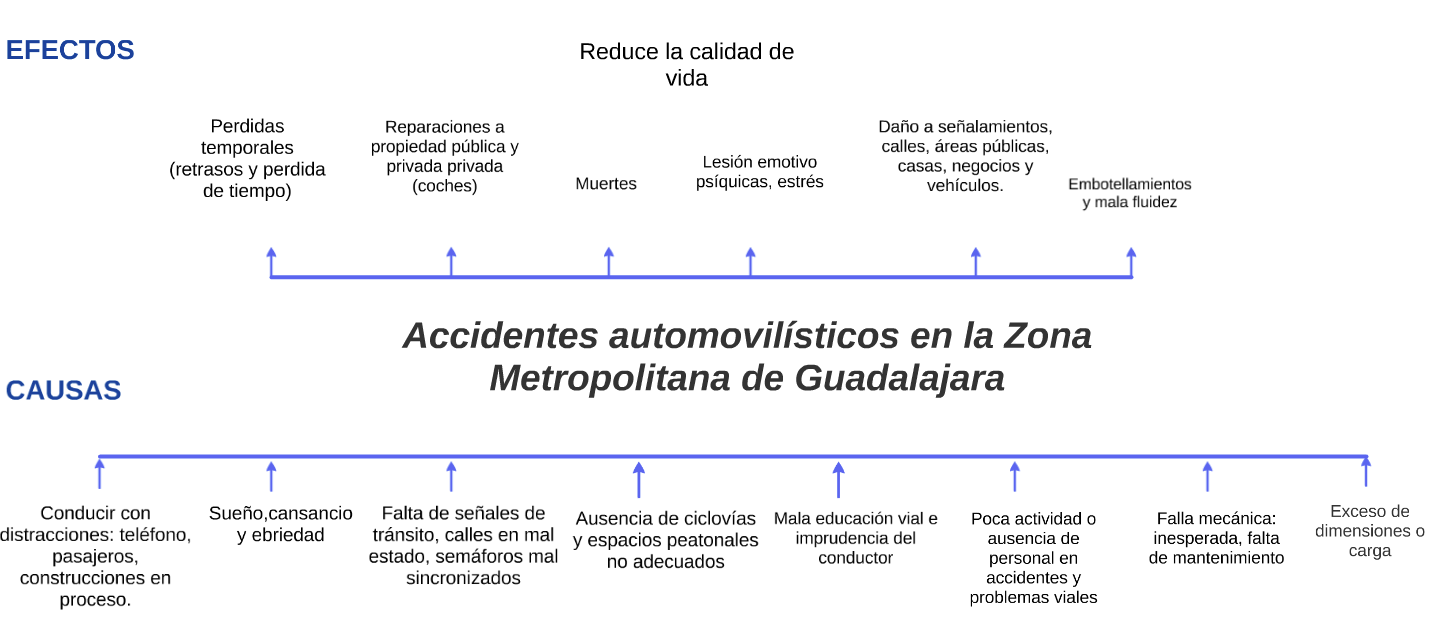
\includegraphics[width=1\textwidth]{resources/img/arbol_de_problemas.png}
	\caption{\label{fig:arbol} Árbol de problemas. Fuente: Elaboración propia.}
    \end{figure}

Las consecuencias que conlleva el problema de los accidentes automovilísticos en una zona tan transitada como lo es la Zona Metropolitana de Guadalajara van desde, daños menores como podrían ser los embotellamientos que impiden la fluidez vehicular y que a su vez ocasionan pérdidas menores temporales como son los retrasos y las pérdidas de tiempo de los conductores, lesiones emotivo-psíquicas y estrés, daños a los señalamientos, calles, áreas públicas o bien lleva a daños aún más graves como lo es la muerte. Efectos que llevan a la población a una disminución de su calidad de vida.

\newpage
\section{Objetivos del proyecto}\label{sec:objs}

En esta sección se plantean los objetivos del proyecto usando como base el
árbol de problemas (figura \ref{fig:arbol}). La intención es usar este árbol para generar
de forma análoga un árbol de objetivos. Esta metodología nos permite garantizar que
el planteamiento de los objetivos y soluciones está completamente alineado a la identificación
de los problemas. 

	\begin{figure}[H]\centering
	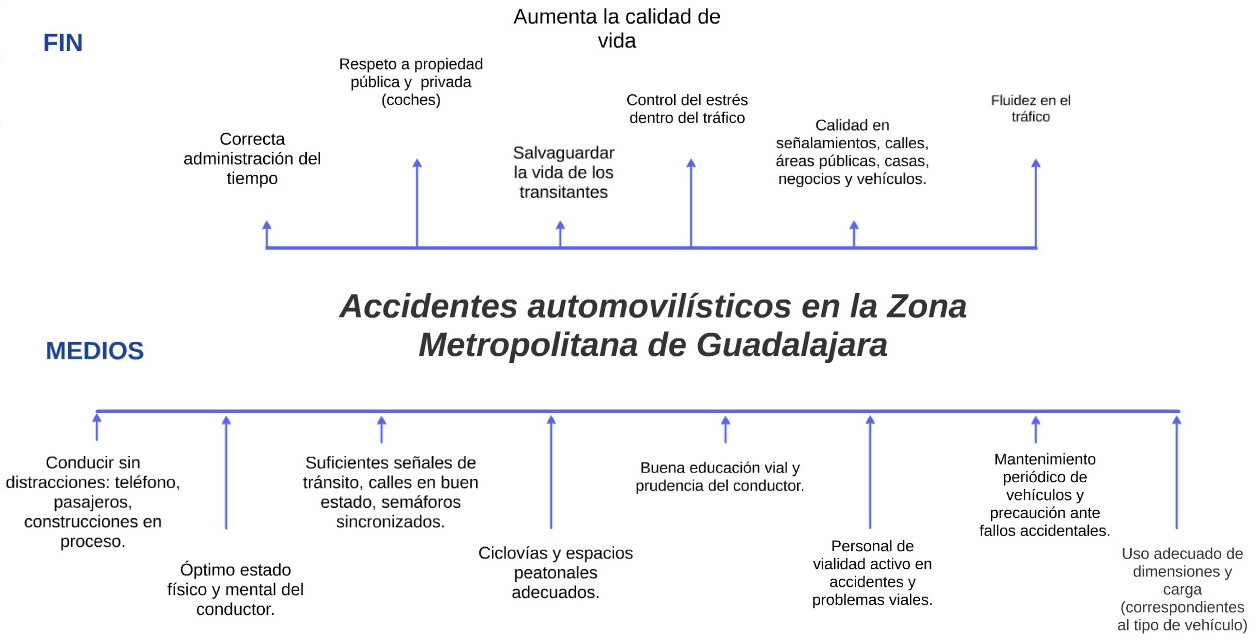
\includegraphics[width=1\textwidth]{resources/img/arbol_de_objetivos.png}
	\caption{\label{fig:arbol_obj} Árbol de objetivos. Fuente: Elaboración propia}
    \end{figure}


\subsection{Objetivo general}\label{subsec:general-objs}

Usando como referencia el árbol de objetivos (figura \ref{fig:arbol_obj}) presentado anteriormente, se propone el siguiente objetivo general:

\forceindent \textit{Mejorar la calidad de vida de los ciudadanos a través de la disminución de accidentes automovilísticos letales en la
Zona Metropolitana de Guadalajara.}

El componente medular de este objetivo reconoce que parte del bienestar social es afectado directamente por los accidentes automovilísticos. Este problema tiene el potencial de agravarse sustancialmente con el crecimiento urbano de la ZMG si no se toman las medidas y políticas adecuadas. En este sentido, se pretende analizar información pública disponible para encontrar la relación entre los accidentes viales y las acciones que se pueden llevar a cabo de forma preventiva. Entre estas acciones se identifican políticas públicas y programas sociales con la intención de generar un impacto positivo y benéfico para la sociedad. 

Actualmente se tiene evidencia de casos de éxito respecto a programas sociales que pretenden reducir los accidentes viales de una causa en particular. Dentro de estos casos, destaca el programa "Salvando Vidas", coordinado por la Secretaría de Movilidad, en donde se atiende de forma exclusiva el consumo de alcohol indebido por conductores de vehículos.

\subsection{Objetivo específico}\label{subsec:specific-objs}

Se propone el siguiente objetivo específico:

\forceindent \textit{Disminuir el número de accidentes automovilísticos letales en la Zona Metropolitana de Guadalajara mediante un esquema de incentivos orientado al uso apropiado del celular.}

Este objetivo se deriva directamente de la parte inferior del árbol en la figura \ref{fig:arbol_obj}. La intención es atender de forma particular y precisa una de las causas más relevantes de la problemática. Esto con el fin de generar un impacto de alto grado y contribuir de una forma más significativa al objetivo general. En particular, se seleccionó este objetivo específico puesto que el uso inadecuado de tecnología celular en zonas urbanas ha presentado una tendencia alcista alarmante.


\newpage
\section{Análisis de los participantes}\label{sec:participants}

El alcance de este documento se limita a la Zona Metropolitana de Guadalajara. Tal zona está integrada por varios municipios, los cuales conforman el área urbana en su conjunto y comparten infraestructura relevante. Los incidentes viales afectan a la "zona urbana" de forma agregada; por esta razón la problemática a tratar trasciende al orden de gobierno municipal. En este sentido, el siguiente orden de gobierno inmediato es el Estado de Jalisco, en el cual se identifican varios participantes. Por otra parte, la naturaleza del problema tiene una orientación pública significativa. En este caso los ciudadanos pertenecientes a la ZMG están involucrados de forma directa. 

En la siguiente tabla se desglosan los participantes:

\begin{table}[H]\centering
\begin{tabular}{l r}
\hline
Participantes & Competencia \\
\hline\hline
Secretaría de Movilidad & Estatal \\
Instituto de Movilidad y Transporte & Estatal \\
Secretaría de Infraestructura y Obra Pública & Estatal \\
Secretaría de Planeación y Administración Financiera & Estatal\\
Ciudadanos & Público \\

\hline
\end{tabular}
\end{table}

\subsection[SEMOV]{Secretaría de Movilidad del Estado de Jalisco}\label{subsec:semov}

La Secretaría de Movilidad (SEMOV) es la autoridad en materia de tránsito y vialidad del Estado de Jalisco. Son los encargados de la seguridad y calidad en el desplazamiento de vehículos dentro de la entidad. 

\subsection[IMTJ]{Instituto de Movilidad y Transporte del Estado de Jalisco}\label{subsec:imtj}

El Instituto de Movilidad y Transporte es un organismo público y descentralizado del Estado de Jalisco cuyo objetivo principal es el de promover la movilidad sustentable. Este instituto se encarga de proponer e implementar actividades para eficientar el transporte. Tiene la facultad de emitir opinión técnica a la SEMOV. 

\subsection[SIOP]{Secretaría de Infraestructura y Obra Pública del Estado de Jalisco}\label{subsec:siop}

La Secretaría de Infraestructura y Obra Pública (SIOP) se encarga del desarrollo, proyección y construcción de obras públicas en el Estado de Jalisco. 

\subsection[SEPAF]{Secretaría de Planeacion y Administracion Financiera de Jalisco}\label{subsec:sepaf}
La Secretaría de Planeación y Administración Financiera (SEPAF) es responsable de garantizar que se destinen los bienes y recursos estatales a las acciones que son prioridad en la planeación y desarrollo del Estado. 

\newpage

\section{Alternativas de solución}\label{sec:alternatives}

% * <rohdzmota@gmail.com> 2018-02-17T00:23:06.435Z:
% 
% Definir un indicador para el problema central y 3 indicadores para el específico.
% Considerar efectos quantificables: 
% * vidas salvadas (monetización)
% * costo promedio de siniestros (personales, infraestructuras, tiempo en embotellamiento)
% * numero de colisiones
% * indicador respecto a población afectada. 
% ^.

\subsection{Metodologías}

\subsection{Situación actual}\label{subsec:actual}

Actualmente se puede apreciar una disminución en el número de accidentes viales por consumo de alcohol, debido a una política para identificar el uso y consumo ilegal de bebidas alcohólicas al conducir.
Por otro lado, a partir del 2015 el número de accidentes automovilísticos letales donde no influye el consumo de alcohol ha comenzado a aumentar. Esto puede ser producto de la reciente alta adopción de tecnologías celulares en la Zona Metropolitana de Guadalajara. En el año 2015 el porcentaje de usuarios de tecnología celular en Jalisco
era del 76.32\%. Esta cifra aumentó a 81.80\% en 2016. La figura \ref{fig:tipo_celular} muestra la
proporción de celulares comúnes y smartphones.


	\begin{figure}[H]\centering
	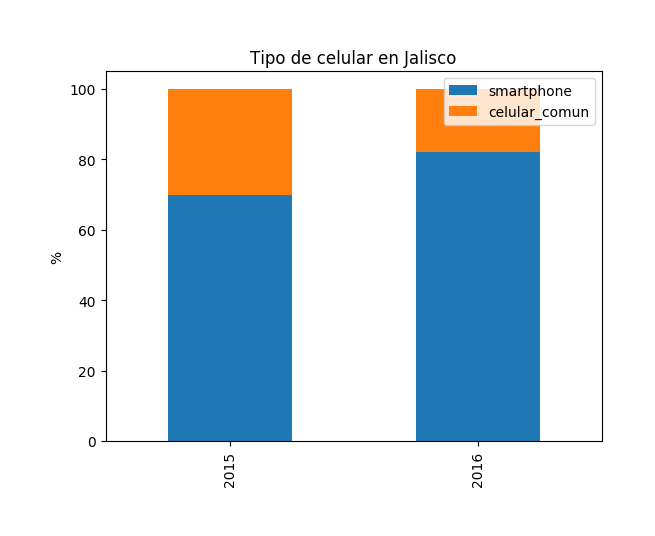
\includegraphics[width=0.6\textwidth]{resources/img/tipo_de_celular.png}
	\caption{\label{fig:tipo_celular} Crecimiento del Smartphone. Fuente: Elaboración propia}
    \end{figure}

La adopción de smartphones ha aumentado durante el periodo del 2015 al 2016 de un
69.8\% hasta un 82.2\%. En recientes estudios, la Organización Mundial de la Salud ha identificado
el uso del celular como un alto factor de riesgo al conducir debido a que genera distracciones
visuales, cognitivas, físicas y auditivas.

Por otra parte, la Secretaría de Movilidad identificó en 2016 el porcentaje de conductores afectados
por distracciones de celular en distintos municipios pertenecientes a la Zona Metropolitana de Guadalajara.
El promedio de la Zona indica que al menos 60\% de los conductores se ven afectados por este tipo
de distracciones al conducir.

	\begin{figure}[H]\centering
	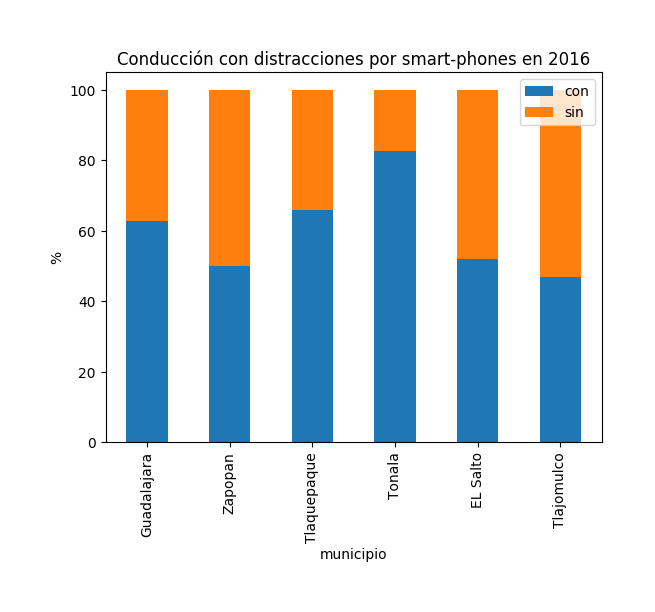
\includegraphics[width=0.6\textwidth]{resources/img/manejo_con_celular.png}
	\caption{\label{fig:manejo_celular} Uso de celular al conducir. Fuente: Elaboración propia con informacion de SEMOV}
    \end{figure}

Tomando en consideración que la adopción de Smartphones
también presenta una tendencia a la alta y está fuertemente correlacionada con accidentes automovilísticos,
la seguridad vial puede verse afectada de forma relevante.

	\begin{figure}[H]\centering
	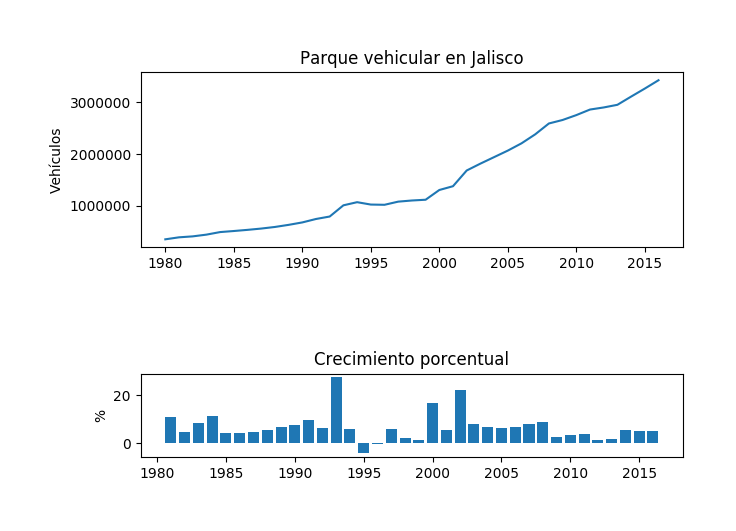
\includegraphics[width=1\textwidth]{resources/img/parque_vehicular.png}
	\caption{\label{fig:parque_vehicular} Vehículos en circulación. Fuente: Elaboración propia}
    \end{figure}

\subsubsection{Definición de indicadores}

Los indicadores nos permiter medir el desempeño del proyecto bajo distintos escenarios.
Respecto al objetivo general, se propone el siguiente indicador:

\begin{itemize}
	\item \textbf{Accidentes automovilísticos letales por año}: número absoluto de accidentes automóvilisticos
con al menos una muerte involucrada.
\end{itemize}

La disminución del valor de este indicador se relaciona de forma directa con la intención propuesta en el objetivo general.

Para el objecto particular se proponen:

\begin{itemize}
	\item \textbf{Pocentaje de usuarios que manejan con distracciones}: actualmente 60\% de los conductores manejan con
distracciones relacionadas al uso de celular.
	\item \textbf{Número de muertes en accidentes automovilísticos que involucren uso de celular}: cerca del 70\% de los
accidentes automovilísticos son generados por uso inapropiado de celular.
	\item \textbf{Ahorro estimado}: la reducción de siniestros tiene beneficios económicos para la población
afectada.
\end{itemize}

Se puede apreciar que los indicadores representan de forma cuantitativa el cumplimiento del objetivo específico.
En el caso particular de los primeros dos indicadores se deberá logarar una disminución. Mientras que el último
indicador debería aumentar.

\subsubsection{Pronóstico: Adopción de tecnología celular}

Se propone usar un modelo de la familia exponencial para pronosticar la adopción de tecnología celular en el Estado
de Jalisco. Asumimos que el porcentaje de adopción a nivel Estado es igualmente representativo para la Zona
Metropolitana de Guadalajara puesto que esta consta de varios municipios relevantes del mismo y
puede ser considerado como una muestra significativa.

El modelo exponencial propuesto en esta sección debe cumplir con las siguientes características:
\begin{itemize}
	\item Comportamiento asintótico respecto a $y=100$, puesto que se estan manejando porcentajes.
	\item Relación no lineal respecto al tiempo ya que se está modelando la adopción de una tecnología.
\end{itemize}

La siguiente figura ilustra algunos ejemplos de comportamiento exponencial:

	\begin{figure}[H]\centering
	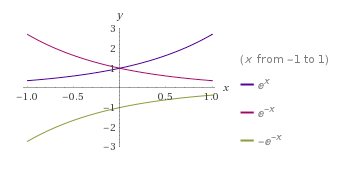
\includegraphics[width=0.6\textwidth]{resources/img/modelo_exp.png}
	\caption{\label{fig:exponential_behaviour} Comportamiento Exponencial. Fuente: Elaboración propia}
    \end{figure}

Por lo tanto, se busca un modelo de la siguiente forma:

\begin{equation}
f(x) = -\alpha e^{-\beta x} + 100
\end{equation}

Donde $\alpha$ y $\beta$ son parámetros de ajuste según el contexto del problema.

En el caso de porcentaje de usuarios de telefonía móvil general sabemos que en 2015 se tenía 76.32\% de usuarios y
en 2016 81.8\%. Por lo tanto, se buscaron los parámetros tales que:

\begin{align*}
f_g(0) = 76.32 \\
f_g(1) = 81.8
\end{align*}

Siguiendo la misma metodología se determinaron los parámetros para el crecimiento del uso de smartphone de tal forma
que se cumpliera:

\begin{align*}
f_s(0) = 69.8 \\
f_s(1) = 82.2
\end{align*}

Los resultados:

\begin{align*}
f_g(x) = -23.68e^{-0.26321x}+100 \\
f_s(x) = -30.2e^{-0.52864x}+100
\end{align*}

Con estos modelos se crea un pronóstico para los siguientes 3 años (6 años a partir del 2015).

	\begin{figure}[H]\centering
	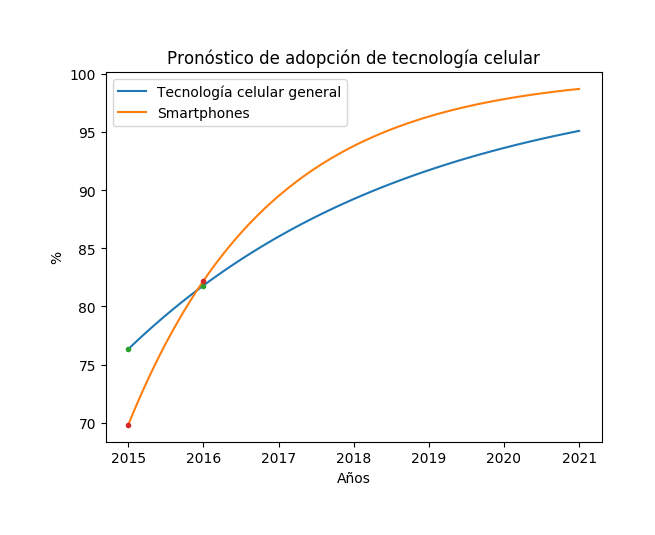
\includegraphics[width=0.6\textwidth]{resources/img/pronostico_adopcion.png}
	\caption{\label{fig:pron_adp} Pronóstico de tasas de adopción. Fuente: Elaboración propia}
    \end{figure}

Los resultados indican que a finales del 2021 aproximadamente 95\% de los habitantes del Estado
tendrán tecnología celular disponible y 98.73\% de estos usuarios tendrán un Smartphone.

Combinando estos pronósticos es posible determinar el porcentaje de la población expuesta al
uso de Smartphones.

	\begin{figure}[H]\centering
	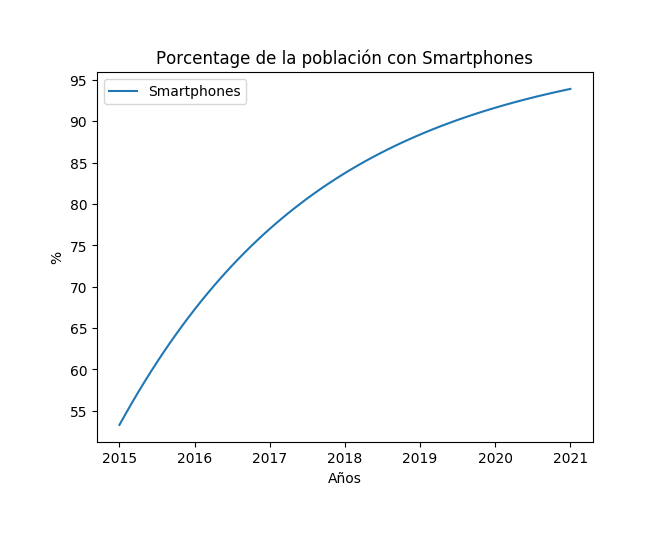
\includegraphics[width=0.6\textwidth]{resources/img/smartphone_usage.png}
	\caption{\label{fig:smart_usage} Uso del Smartphone. Fuente: Elaboración propia}
    \end{figure}

\subsubsection{Pronóstico: Crecimiento del parque vehicular}

Para pronosticar el crecimiento del parque vehicular en el Estado se usa
un modelo con bases probabilísticas que nos permite generar distintas
simulaciones e identificar la tendencia media.

En este caso se usó como base el crecimiento histórico generado en los
últimos 20 años. La siguiente figura representa de forma visual el
resultado de 200 simulaciones para los siguientes 3 años.

	\begin{figure}[H]\centering
	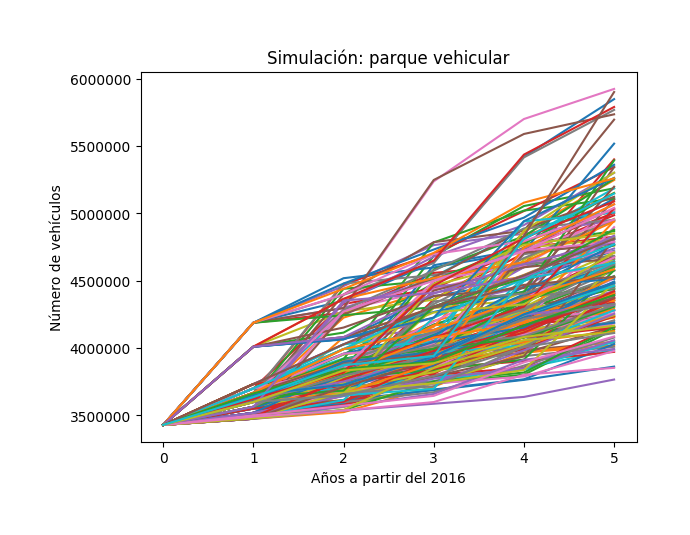
\includegraphics[width=0.6\textwidth]{resources/img/vehicle_forecast_img.png}
	\caption{\label{fig:vehicle_forecast} Pronóstico de vehículos en circulación. Fuente: Elaboración propia}
    \end{figure}

La simulación indica que para el 2021 se estiman 4,679,213 vehículos en circulación.
En el 2016 se reportaron 7 accidentes por cada 1000 vehículos en circulación y de tales accidentes el
2.26\% fueron fatales.


\subsubsection{Pronóstico: Manejo con distracciones}

En 2016, el Instituto de Información Estadística y Geográfica de Jalisco indentificó que
aproximadamente 60\% de los conductores de automóvil manejan con alguna distracción
relacionada con el uso de Smartphones. Para modelar la dinámica de esta propoción de conductores podemos
asumir que existe una relación proporcional con el porcentaje de usuarios de Smartphone.

Por lo tanto, se define la siguiente relación lineal:

\begin{equation}
\delta_t = k_t s_t
\end{equation}

Donde $\delta_t$ representa el porcentaje de conductores que manejan con distracciones de Smartphone,
$k_t$ es un factor proporcional y $s_t$ es el porcentaje de usuarios de Smartphone. En el caso más
simple $k_t = k$ es constante.


Sabemos que $s_{2016} = 67.23$ y por lo tanto $k_{2016} = k = 60/67.23 = 0.892459$.

Usando los datos del pronóstico anterior, se genera el pronóstico para $\delta_t$.

	\begin{figure}[H]\centering
	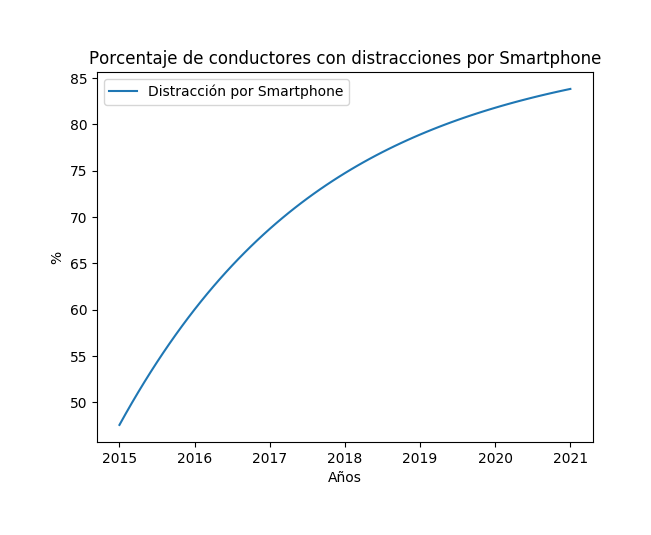
\includegraphics[width=0.6\textwidth]{resources/img/distraction.png}
	\caption{\label{fig:distr} Distracciones generadas por Smartphones. Fuente: Elaboración propia}
    \end{figure}

Para el 2021, usando las tendencias y supuestos mostrados en esta sección, se estima
que aproximadamente el 83.81\% de los conductores manejan con distracciones generadas
directamente por un smartphone.

Esta cifra es particularmente alarmante puesto que actualmente la SEMOV identifica
que cerca del 70\% de los percances viales son generados por usar el celular de
forma indebida. La siguiente figura muesta los resultados generales referentes a la adopción de
tecnología celular.

	\begin{figure}[H]\centering
	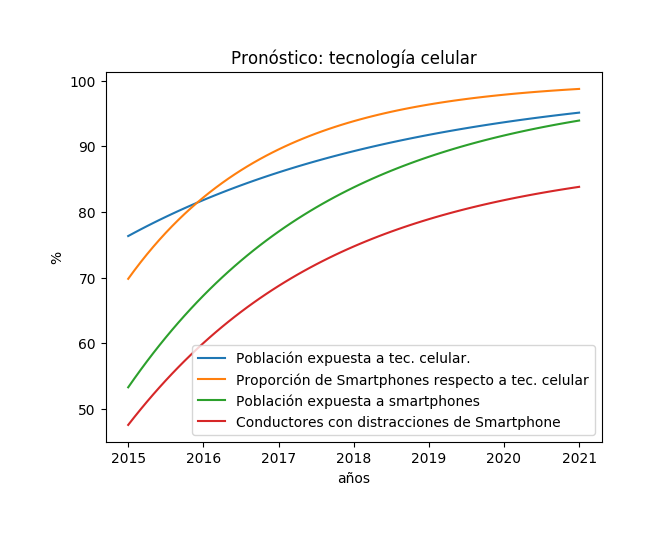
\includegraphics[width=0.6\textwidth]{resources/img/smartphone_complete_forecast.png}
	\caption{\label{fig:compare_forecast} Pronóstico General. Fuente: Elaboración propia}
    \end{figure}

\subsubsection{Pronóstico: Accidentes por uso de smartphone}

Dado el pronóstico del crecimiento del parque vehicular y el porcentaje de conductores expuestos a
distracciones con Smartphones, es posible calcular el número de accidentes generados particularmente
por el uso de esta tecnología al conducir. Por estadísticas de la SEMOV, sabemos que en 2016 se registraron 7
accidentes automovilísticos por cada 1000 vehículos en circulación. Adicionalmente, un estudio realizado por este
mismo organismo sugiere que actualmente el 70\% de los siniestros son generados por una distracción directa de la
tecnología celular. En este sentido entonces podemos asumir 4.9 accidentes por cada 1000 vehículos en circulación.

Por lo tanto, se propone la siguiente fórmula para calcular el número de accidentes viales generados por el uso
de celular, basado en datos del 2016:

\begin{equation}
accidentes_{t} = \frac{4.9 * vehiculos_t * \delta_t}{1000 * 0.6}
\end{equation}

Usando esta propuesta obtenemos los siguientes resultados:

	\begin{figure}[H]\centering
	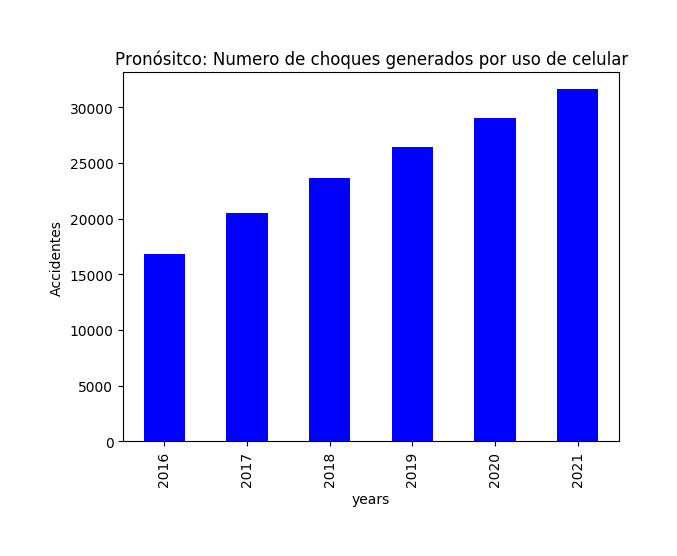
\includegraphics[width=0.6\textwidth]{resources/img/smart_accidents.png}
	\caption{\label{fig:smart_accidents} Accidentes generados por SmartPhones. Fuente: Elaboración propia}
    \end{figure}

Se puede apreciar la tendencia alcista. De estos resultados, se espera que al menos 2.26\% de tales accidentes sean
fatales.

\subsubsection{Pronóstico: Muertes derivadas por uso de Smartphones}

Utilizando los datos de la SEMOV sabemos que al menos el 2.26\% de los accidentes viales
son fatales (implica al menos 1 muerte). No obstante, en los últimos años se ha mostrado una tendencia alcista. Por 
este motivo, es prudente realizar este análisis con una tasa del 3\%.

La siguiente gráfica ilustra la evolución del número de accidentes viales con repercusiones fatales:  

	\begin{figure}[H]\centering
	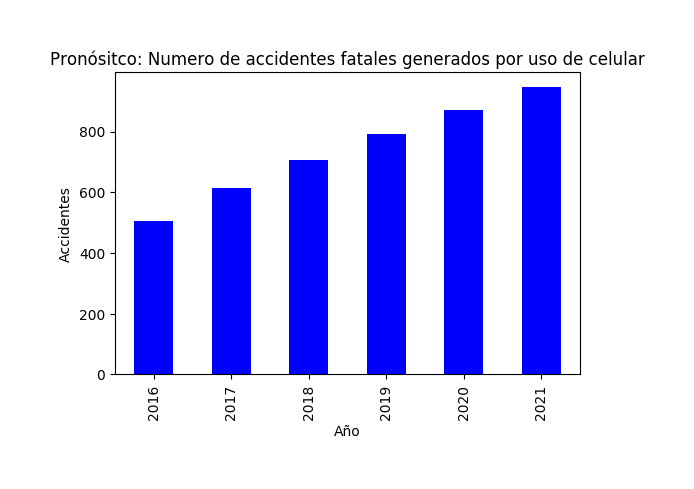
\includegraphics[width=0.6\textwidth]{resources/img/smart_accidents_deaths.png}
	\caption{\label{fig:prono_accidentes_fatales} Número de accidentes fatales generados por uso de celular. Fuente: Elaboración propia}
    \end{figure}

En general entre el 2018 y el 2021 se tendrían al menos 3317 muertes, suponiendo que cada accidente fatal solamente 
conlleva a una persona fallecida (caso optimista). 

\subsection{Situación con proyecto}

El proyecto pretende generar un alto impacto en la disminución de la sinestralidad generada principalmente por el uso
de Smartphones. No obstante, la tendencia de carácter exponencial que muestra la adopción de esta tecnología en la
población de interés genera un alto reto.

Se trata no solo de un fenómeno extraordinario o moda, sino de una aparente necesidad de comunicación y dependencia a estos dispositivos, de manera que se vuelve parte de la rutina social, incluso al conducir. Por lo que una intervención se vuelve necesaria.  

\subsubsection{Pronóstico: Manejo con distracciones}

En particular la implementación del proyecto debería cambiar la constante $k_t$ por año (en la sección anterior
se mostraron los resultados invariantes). Esta constante representa la relación entre los usuarios activos de Smartphones
y el porcentaje de conductores con distracciones por esta tecnología.

Bajo un escenario conservador, podríamos esperar que los efectos del proyecto tengan una relación lineal en el tiempo
con $k_t$. La razón de cambio mínima esperada es de $0.02$ unidades.

\begin{equation}
k_{t} = k - 0.02 * t
\end{equation}

Con estos supuestos, el pronóstico del porcentaje de conductores con distracciones de smartphone cambiaría de la
siguiente forma:

	\begin{figure}[H]\centering
	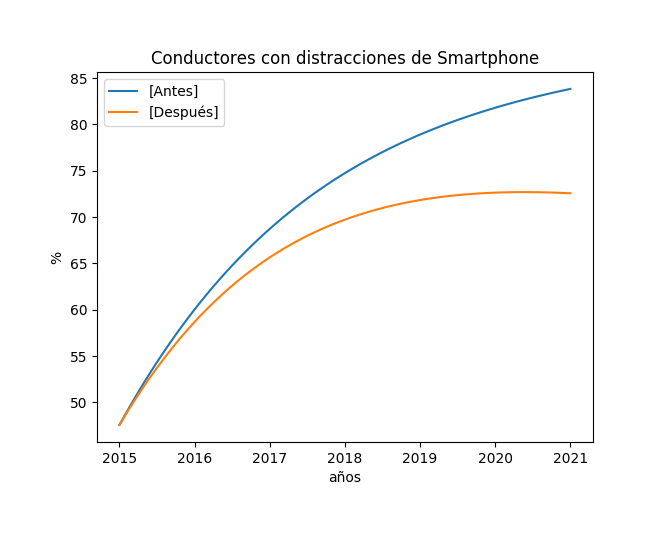
\includegraphics[width=0.6\textwidth]{resources/img/distraction_compare_img.png}
	\caption{\label{fig:smart_accidents_compare} Distracciones por Smartphones al conducir. Fuente: Elaboración propia}
    \end{figure}

De esta manera, podemos decir que con un cambio mínimo del 0,02 se espera una reducción del 80 por ciento  a un 70 por ciento dentro de los siguientes 4 años.

\subsubsection{Pronóstico: Accidentes por uso de smartphone}



	\begin{figure}[H]\centering
	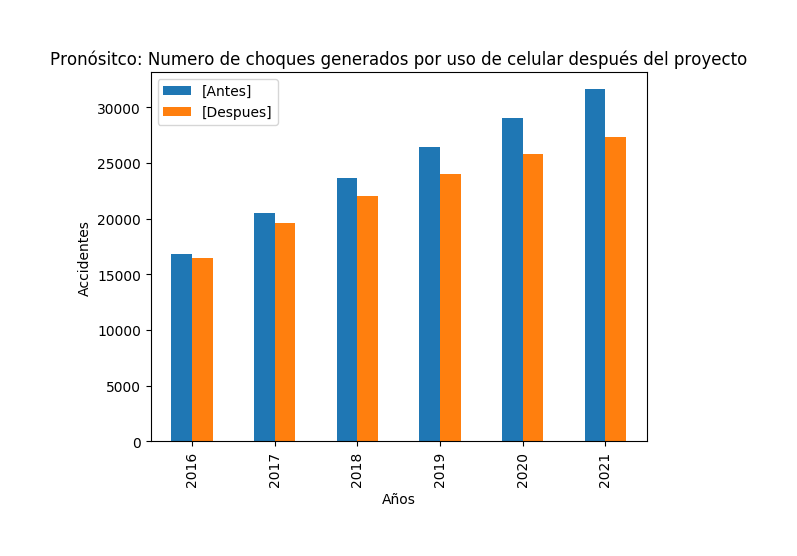
\includegraphics[width=0.6\textwidth]{resources/img/smart_accidents_after.png}
	\caption{\label{fig:smart_accidents_after} Accidentes viales. Fuente: Elaboración propia con información de la SEMOV}
    \end{figure}
Como se puede observar en la $figura 18$ el número de choques generados por el uso de Smartphone implementando el proyecto, provoca un desaceleramiento dentro de la tendencia alcista. Impactando directamente al número de accidentes víales. De manera que para el 2021 se alcance casi la reducción de 5000 accidentes, considerando una postura conservadora a mediano plazo (3 años), sin embargo con el paso de los años esta diferencia se vuelve aun más significativa. 

\subsubsection{Pronóstico: Muertes derivadas por uso de smartphones}

En la sección anterior, se utilizaron datos de la SEMOV ajustados a una expectativa alcista para calcular el número 
de accidentes viales fatales dado la proyección del número de accidentes general. La tasa que se utilizó anteriormente, para representar los accidentes automovilísticos que terminaron al menos con una muerte 
fue del 3\%. En esta sección, mediante la aplicación del proyecto de incentivos para el mejor uso de la tecnología celular se espera tener un impacto positivo que logre reducir la tasa de accidentes viales que terminen en fatalidad al 2\%.

Se obtienen los siguientes resultados:

	\begin{figure}[H]\centering
	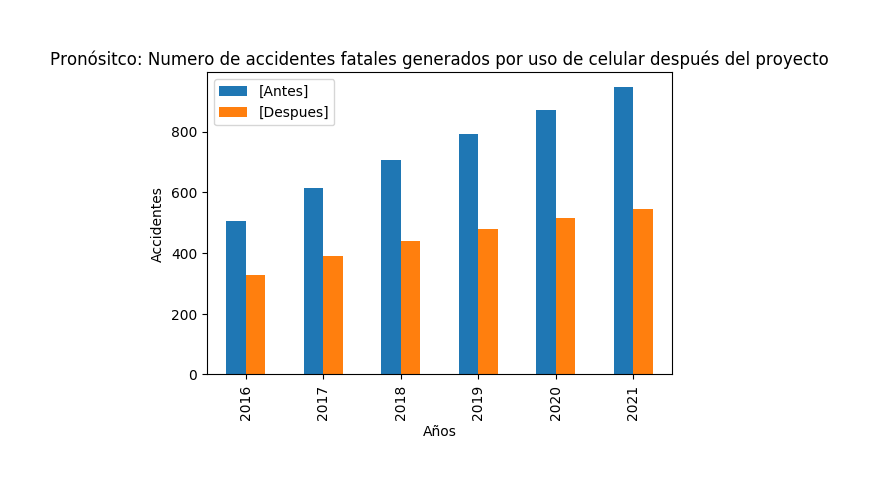
\includegraphics[width=0.8\textwidth]{resources/img/smart_fatal_accidents_after.png}
	\caption{\label{fig:prono_accidentes_fatales_after} Número de accidentes fatales después de proyecto. Fuente: Elaboración propia}
    \end{figure}
    

Con la aplicación del proyecto se estima que el número de muertes provocadas por accidentes automovilísticos entre el periodo de 2018 a 2021 sea de 1982, suponiendo el mejor escenario posible, es decir, una muerte por accidente con categoría fatal, lo que llevaría a una reducción en los próximos 3 años de aproximadamente 1335 muertes, Es decir en solo cuatro años se estaría reduciendo un 33\% los accidentes viales que provocan mortalidad y a su vez una calidad de vida de las personas posiblemente involucradas en el siniestro.


\subsection{Análisis Costo-Beneficio}
% * <rohdzmota@gmail.com> 2018-02-17T00:17:19.479Z:
% 
% Beneficios - Costos > 0  -- rentable, TIR
% 
% ^.


\subsubsection{Costos}

Se estima que con el desarrollo de la app y el esquema de incentivos, al menos el 14\% de los conductores
estén participando de forma activa en el programa durante el primer año y esta cifra aumente 10 puntos porcentuales
por año. 

\textbf{Mercadotecnia y publicidad}
Una vez iniciado el proyecto, va a ser necesario tener un poder de alcance lo suficientemente grande para poder 
De acuerdo a la información proporcionada por un importante publicista y mercadólogo del periódico "El Noroeste", 

\textbf{Desarrollo y mantenimiento de la app}

Hay dos componentes esenciales del proyecto: la aplicación móvil y la infraestructura tecnológica necesaria para
el manejo de datos de forma eficiente. Para reducir costos y complejidad, se propone utilizar en la medida que sea
posible, servicios administrados y frameworks de desarrollo. En particular se contempla usar el ''stack'' de tecnologías
de Google. 

Para la aplicación móvil se está considerando usar el lenguaje de programación de Dart y el ambiente de desarrollo de 
Flutter que permite usar el mismo código para aplicaciones de Android y iOS. A continuación se propone el personal necesario y una estimación de sueldos mensual:  
\begin{itemize}
\item Project manager: \$30,000.00 MXN
\item User Experience Designer: \$25,000.00 MXN
\item Senior Mobile Developer: \$50,000.00 MXN
\item Mid. Mobile Developer: \$30,000.00 MXN
\item Jr Developer: \$20,000.00 MXN
\end{itemize}

El manejo de la infraestructura y servicios en la nube es otra cuestión de suma importancia. Se propone el siguiente equipo para manejo de datos e infraestructura: 
\begin{itemize}
\item Project manager: \$30,000.00 MXN
\item Senior Data Engineer: \$60,000.00 MXN
\item Senir Data Scientist: \$60,000.00 MXN
\item Mid Data Engineer: \$40,000.00 MXN
\item Jr Data Engineer/Scientist: \$30,000.00 MXN
\end{itemize}

En general de forma mensual se pagaría \$ 375,000.00 en sueldos de ingeniería lo cual es \$4,500,000.00 MXN de forma anual. 

\textbf{Almacenamiento y procesamiento de datos en la nube}

-- work in progress --

\textbf{Incentivos}

-- work in progress --


\subsubsection{Beneficios}

-- work in progress --

\textbf{Reducción de accidentes viales}

Con base en la información proporcionada por la Convención de Aseguradores de México, podemos optar por una cifra certera en el costo promedio por accidente, este no depende de ninguna variable, es simplemente por cualquier accidente.

Suponiendo un costo de siniestro promedio de 24,603 MXN (según la Convención de Aseguradores de México) el ahorro
monetario anual sería el siguiente:

	\begin{figure}[H]\centering
	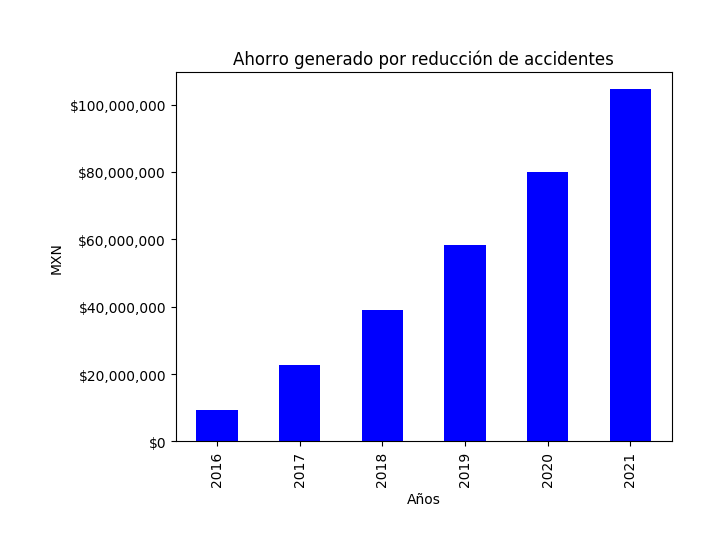
\includegraphics[width=0.6\textwidth]{resources/img/accident_savings.png}
	\caption{\label{fig:accident_savings} Ahorro generado. Fuente: Elaboración propia}
    \end{figure}



Demostrando las gráficas, podemos comparar que los siniestros han incrementado de manera drástica debido a la distracción por el uso de Smart Phone. Concluyendo que el comportamiento del ahorro está en función a la distracción por celulares, entre otras variables que lo determinan. Es por esto que al reducir dicho factor, el gasto por siniestros se verá afectado directamente. 
 
Derivándose en una reducción del gasto y frenando de manera considerable la tendencia alcista de siniestros, como se muestra en el árbol de problemas $figura 5$. Abonando de forma concreta a la reducción (y prevención) de accidentes dentro se la Zona Metropolitana de Guadalajara. 

\textbf{Reducción de muertes}

Uno de los beneficios más apreciables de este proyecto se encuentra en la reducción del número de muertes. En la 
sección anterior (situación con proyecto) se realizaron los pronósticos necesarios para calcular el impacto 
de este proyecto en la disminución de accidentes viales con repercusiones fatales. 

La siguiente gráfica ilustra el número de vidas salvadas por año: 

	\begin{figure}[H]\centering
	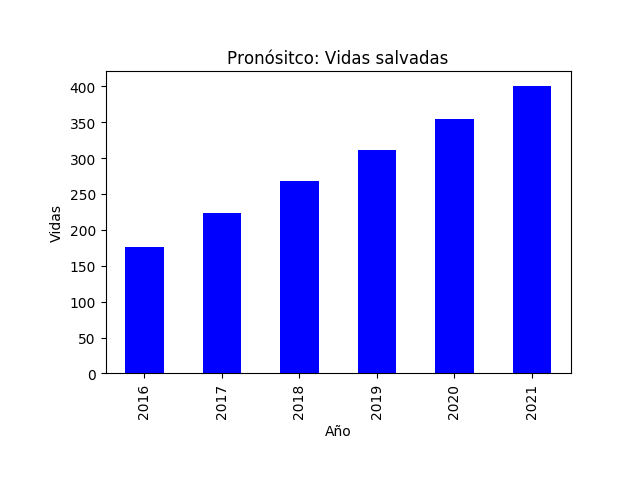
\includegraphics[width=0.6\textwidth]{resources/img/saved_lifes.png}
	\caption{\label{fig:vidas_salvadas} Estimación de vidas salvadas. Fuente: Elaboración propia}
    \end{figure}


Se utiliza el valor estadístico de la vida (\$ 1,687,037.00 MXN) proporcionado por ... para ...

El beneficio monetario resultante es el siguiente:


	\begin{figure}[H]\centering
	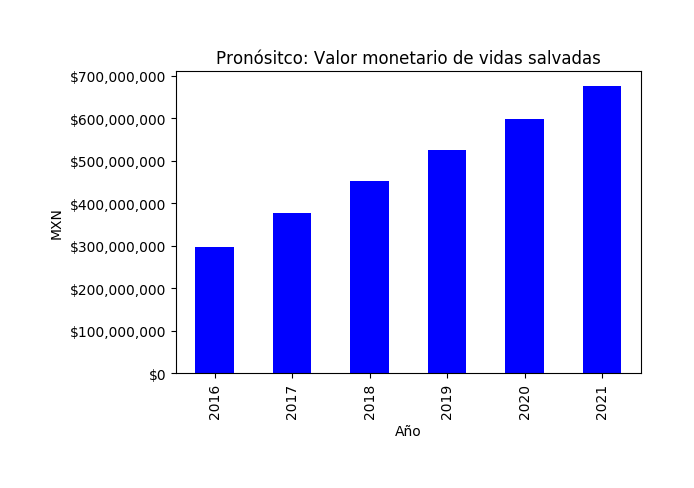
\includegraphics[width=0.6\textwidth]{resources/img/saved_lifes_money.png}
	\caption{\label{fig:vidas_salvadas_dinero} Estimación monetaria de vidas salvadas. Fuente: Elaboración propia}
    \end{figure}

Se puede observar... 

\textbf{Información accionable}

-- work in progress --

\textbf{Rentabilidad}

-- work in progress --

\subsection{Simulación Montecarlo}

\subsection{Análisis de Sensibilidad}

\subsection{Resultados}
% * <rohdzmota@gmail.com> 2018-02-17T00:16:37.605Z:
% 
% Concluir si el proyecto es rentable o no
% 
% ^.

\newpage
\section{Elaboración de la MIR}\label{sec:mir}
[agregar contenido]

\newpage
\section{Conclusiones}\label{sec:conclutions}
[agregar contenido]

\newpage
\section{Bibliografía}\label{sec:references}
[agregar contenido]

\end{document}
